%!TEX root = Main.tex
\documentclass[Main]{subfiles}

\begin{document}

\section{Plan and schedule the necessary activities} 

% TODO:
All activities must be broken down in smaller bit in a Plan-Driven.
This is due to a static hardware setup and no customer to interact with.
\\
\\
The following must be included as activities:
\begin{enumerate}
	\item Validate user requirements
	\item Software design
	\begin{itemize}
		\item HW/SW interfaces
		\item Software architecture
		\item Display driver
		\item Projector driver
		\item Clock and alarm driver
		\item Sound driver
		\item Button driver
	\end{itemize}
	\item Software implementation
	\item Test specification
	\item Integration
	\item Acceptance test
	\item User manual
\end{enumerate}

In Figure \ref{fig:activityPlanning} all the activities are shown with estimated duration and interdependencies. Each activity is given a unique identifier in the top-left box, and a estimated duration in the top-right box. 
The four middle boxes shows the first and last start and stop times in weeks. 
The lower-left box shows time available for each activity and the lower-right box shows the slack available slack time. 
It is easy to find the critical path, by following the activities with zero slack time, which has been marked with thicker arrows.

\begin{figure}[hbtp]
\centering
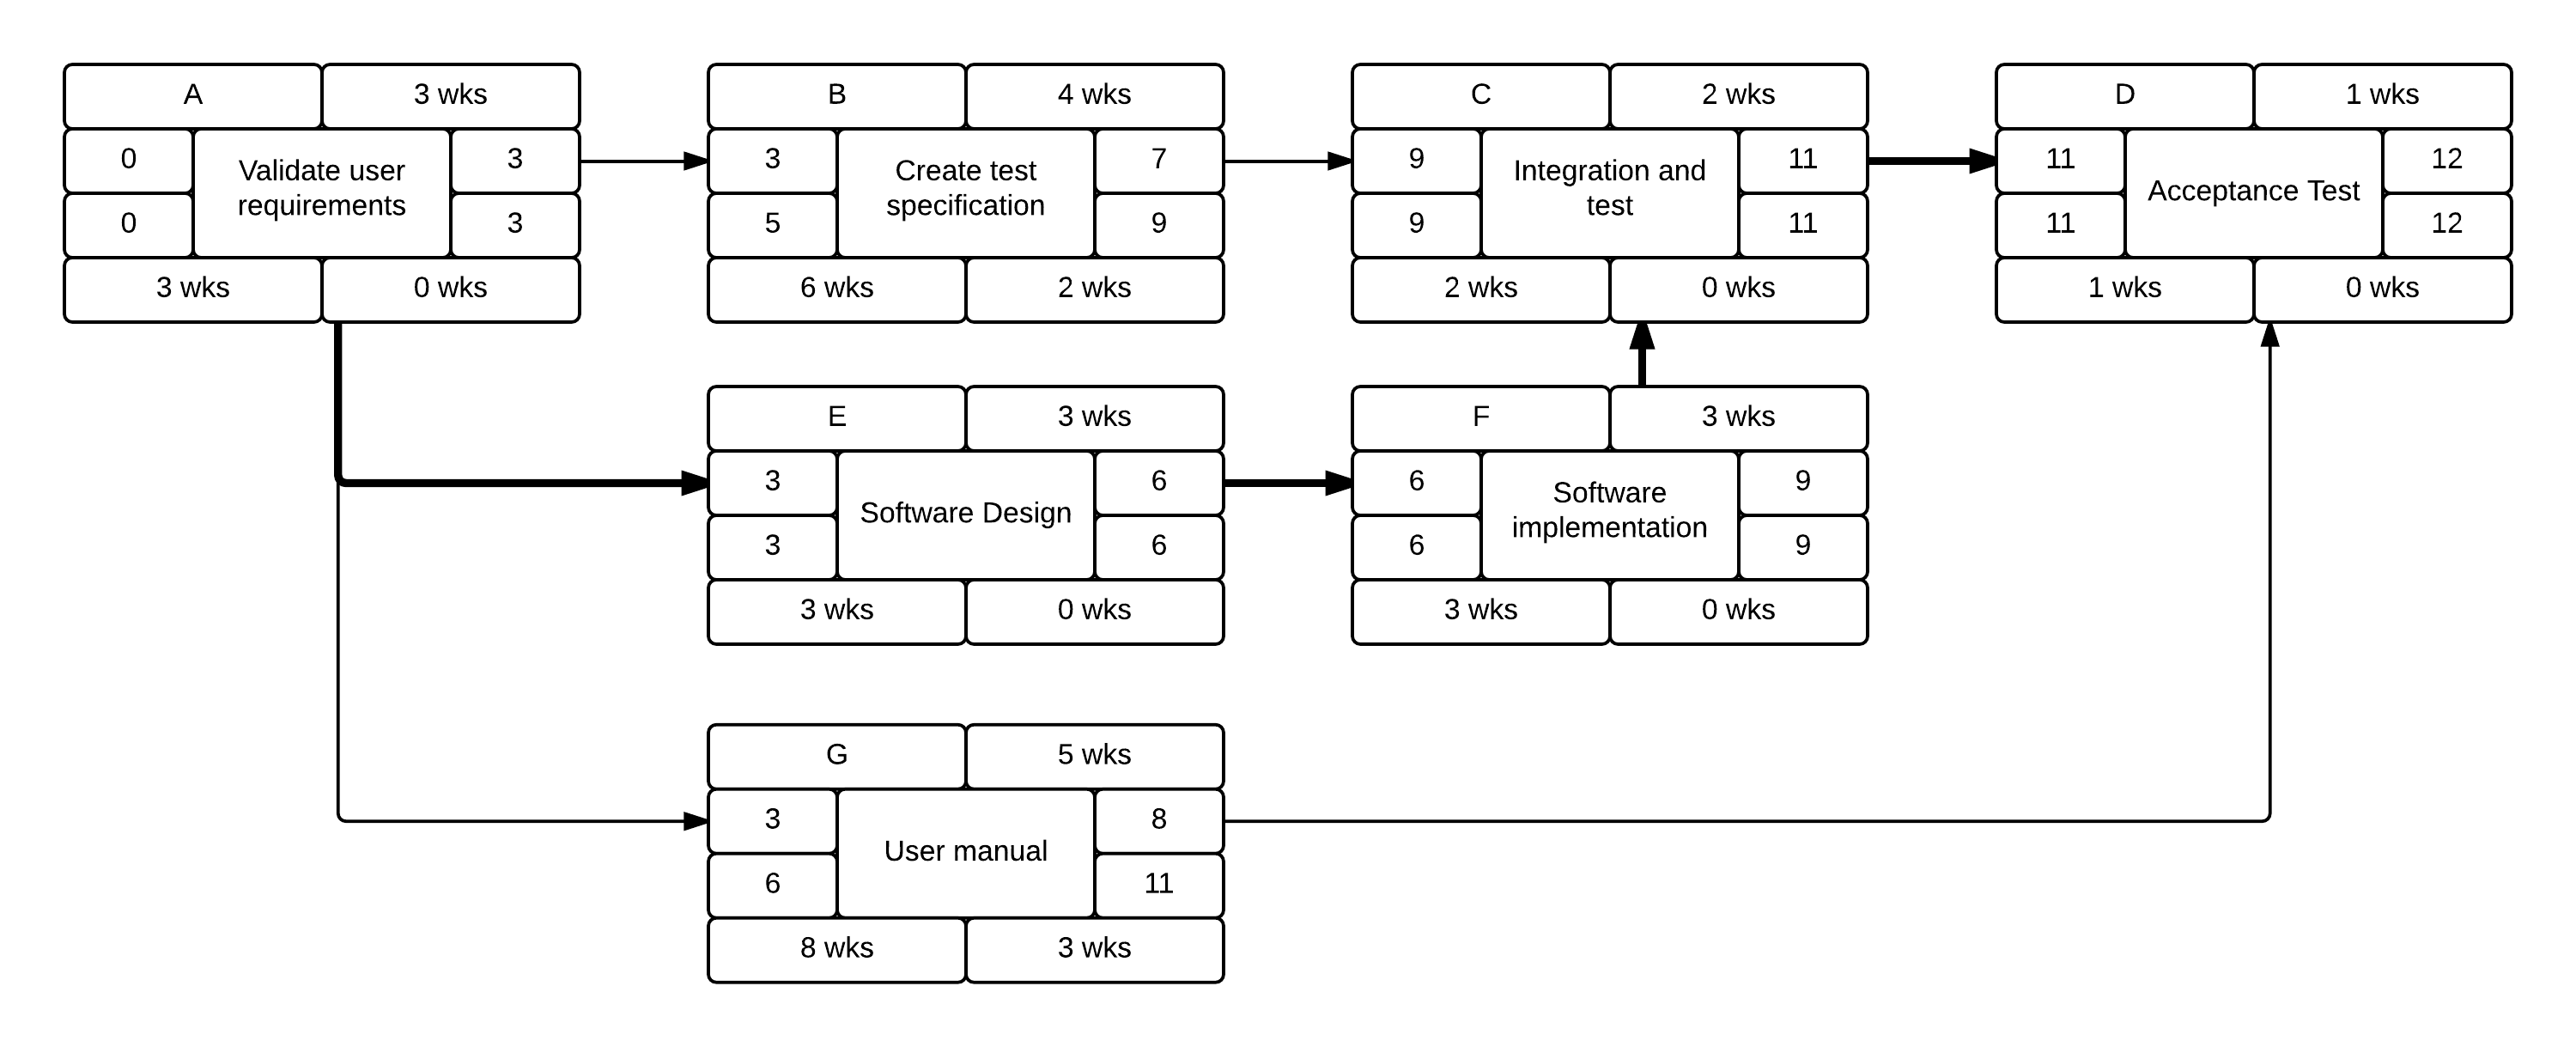
\includegraphics[width=\linewidth]{ActivityPlanning}
\caption{Activity planning}
\label{fig:activityPlanning}
\end{figure}


\end{document}